\section{Thu, Aug 2, 2018}

Got a book yesterday in the mail. The journals of William Clayton, Joseph Smith's
personal secretary. It's an interesting read for sure. I'm excited to have it, I
already began reading through the Nauvoo period, very interesting book.

\begin{figure}[h!]
  \centering
  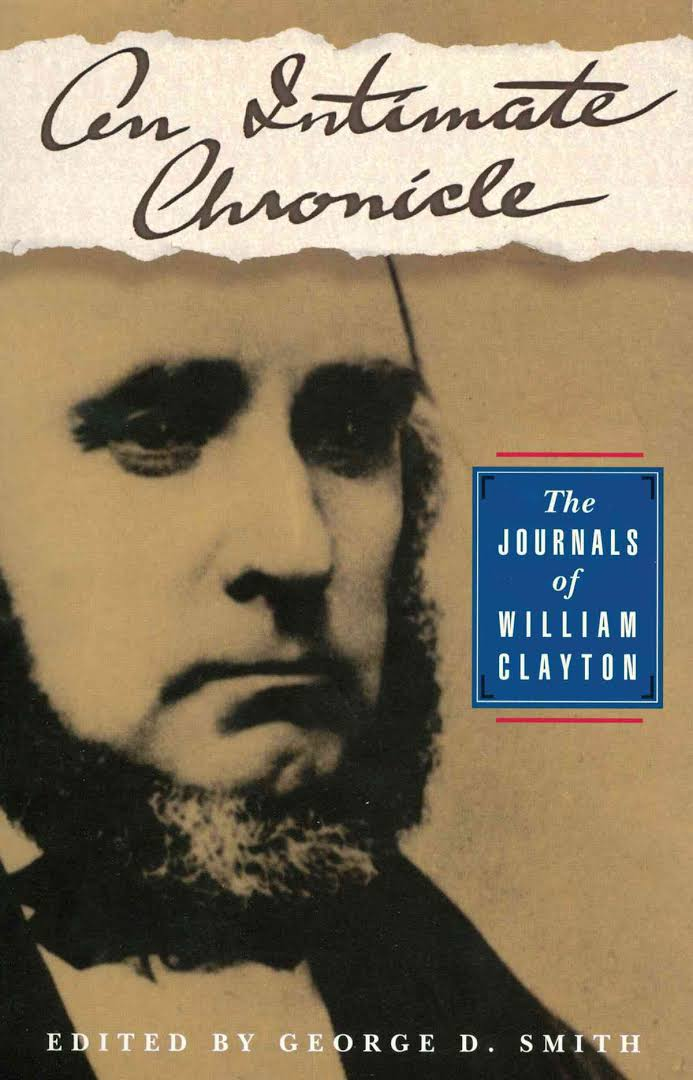
\includegraphics[width=0.5\linewidth]{2018/images/clayton.jpg}
  \caption{An Intimate Chronicle: The Journals of William Clayton}
  \label{fig:clayton}
\end{figure}

It's another day, waiting for bills to go through is not the easiest thing in the
world. We live in a world where transactions can occur instantly. Yet when a person
pays for a bill, it takes forever it seems to go through. What's up with that? I
don't get it. I don't understand any of it. Such an odd weird life to be living in a
times. We have come so far in advancements in technology, and yet here we are waiting
for something to go through. So very very odd.

Oh well, it is life as it would seem to be...I guess. Whatever the case, here we are
just trying to live another day and get by. There's nothing wrong with any of that,
is there? No, I didn't think there would be. I mean, let's face it. Life comes and
goes long after we are gone. We will always be remembered in a place where we were
the most happy, the most plesent of thoughts. There is no reason to think otherwise.
Is that not what people wish to remember about people? The good memories, the good
thoughts upon which they are able to exist? Yes, something along those lines for
sure.

I fear at times, I do not have the adequate knowledge or thought process as those of
old who have gone on before. But I cannot allow it to simply be erased. Whatever I
was in this life is what I was. Whatever I will become in this life, is what I will
become. I cannot change the past. I can only look forward to the future with a
brightness of hope.
